%%%%%%%%%%%%%%%%%%%%%%%%%%%%%%%%%%%%%%%%%%%%%%%%%%%%%%%%%
%
% PRODUCT SPECIFICATION - eParts Services
% Capstone Project - CMU MSE
%
%%%%%%%%%%%%%%%%%%%%%%%%%%%%%%%%%%%%%%%%%%%%%%%%%%%%%%%%%

\documentclass[12pt, a4paper]{article}

% --- PACKAGES ---
\usepackage[T1]{fontenc}
\usepackage[a4paper, top=2.5cm, bottom=2.5cm, left=2.5cm, right=2.5cm]{geometry}
\usepackage[hidelinks,hypertexnames=false]{hyperref}
\usepackage{titling}
\usepackage{fancyhdr}
\usepackage{booktabs}
\usepackage{array}
\usepackage{longtable}
\usepackage{graphicx}
\usepackage{float}
\usepackage{enumitem}

% --- DOCUMENT METADATA ---
\title{Product Specification \\ \vspace{0.5cm} \Large Intelligent Ingestion \& Attribute Prediction System}
\author{eParts Studio Team} 
\date{\today}

% --- HEADER & FOOTER SETUP ---
\pagestyle{fancy}
\fancyhf{}
\fancyfoot[C]{\thepage}
\renewcommand{\headrulewidth}{0pt}
\renewcommand{\footrulewidth}{0pt}

% --- TITLE PAGE CUSTOMIZATION ---
\pretitle{\begin{center}\Huge\bfseries}
\posttitle{\end{center}}
\preauthor{\begin{center}\Large \vspace{1.5cm}}
\postauthor{\\[1cm] \normalsize Client: eParts Services LLC \\[0.5cm] Document Version: 1.2 \end{center}}
\predate{\begin{center}\large}
\postdate{\end{center}\vfill}

% --- DOCUMENT BEGINS ---
\begin{document}
\hypersetup{pageanchor=false}

% --- 1. COVER PAGE ---
\maketitle
\thispagestyle{empty}
\newpage

% --- 2. TABLE OF CONTENTS ---
\pagestyle{fancy}
\hypersetup{pageanchor=true}
\setcounter{page}{1}
\pagenumbering{roman}
\tableofcontents
\newpage
\pagenumbering{arabic}

% --- 3. VERSION HISTORY ---
\section*{Version History}
\begin{tabular}{@{}llp{10cm}@{}}
\toprule
\textbf{Version} & \textbf{Date} & \textbf{Change} \\
\midrule
0.1 & Feb 01, 2026 & Initial draft based on eParts architectural review. \\
0.5 & Feb 10, 2026 & Added detailed functional requirements for Ingestion and ML Service. \\
1.0 & Apr 24, 2026 & Baseline specification for development. \\
1.1 & Jul 23, 2026 & Integrated ETIM classification/enrichment; corrected OCR (Azure Document Intelligence) and ingestion (channels, Azure Blob storage, quarantine). \\
1.2 & Jul 28, 2026 & Pinned the project to ETIM release 10.0 (language EI) for its duration (new constraint C-4); scoped FR-10 accordingly and removed the implied obligation to adopt later ETIM releases. \\
\bottomrule
\end{tabular}

\vspace{1cm}

% --- 4. GLOSSARY ---
\section*{Glossary}
\begin{longtable}{@{}l >{\raggedright\arraybackslash}p{12cm}@{}}
\toprule
\textbf{Term} & \textbf{Definition} \\
\midrule
\endfirsthead
\toprule
\textbf{Term} & \textbf{Definition} \\
\midrule
\endhead
\bottomrule
\endfoot
\bottomrule
\endlastfoot
PIMS & Product Information Management System. The system where the final product catalog data lives (downstream source of truth). Approved output is written to PIMS keyed by ETIM identifiers. \\
\addlinespace
Ingestion Gateway & The entry point for raw supplier files (CSV and PDF, via SFTP or direct upload; Email and web sources are planned) into the system. \\
\addlinespace
Confidence Score & A numerical value (0-1) assigned by the ML model indicating the probability that a predicted attribute is correct. \\
\addlinespace
Human-in-the-Loop & A workflow where low-confidence ML predictions are routed to a human operator for manual verification. \\
\addlinespace
ETIM & A standardized technical product-classification model (product groups $\rightarrow$ classes $\rightarrow$ features $\rightarrow$ allowed values / units) used to normalize and enrich supplier attributes. It is reference data layered onto the pipeline, not supplier product data. This project targets ETIM release \textbf{10.0}, language \textbf{EI}, and does not adopt later releases (C-4). \\
\addlinespace
Canonical Table & A standardized, intermediate database schema used to normalize disparate supplier formats before prediction. Its attribute rows are ETIM-keyed (class / feature / value), while the original supplier values are always retained as evidence. \\
\end{longtable}
\newpage

% --- 5. MAIN DOCUMENT ---

\section{Introduction}

\subsection{Purpose}
The purpose of this system is to automate the ingestion, classification, and attribute extraction of product specifications for eParts Services. Currently, this process is manual, error-prone, and unscalable. This project aims to:
\begin{itemize}
    \item Standardize disparate supplier data formats (PDF, CSV, Email).
    \item Utilize Machine Learning to predict product attributes with confidence scoring.
    \item Implement a "Human-in-the-Loop" workflow to review low-confidence predictions, ensuring high data quality for the PIMS.
\end{itemize}

\subsection{Product Description}
The system is a cloud-native data pipeline composed of three primary stages:
\begin{enumerate}
    \item \textbf{Ingestion \& Normalization:} A gateway that accepts raw files via SFTP or direct upload (Email and web sources planned), validates them, and converts them into a structured intermediate format aligned to the ETIM classification standard. Text-native CSV/PDF are parsed deterministically; datasheet PDFs are OCR'd (Azure AI Document Intelligence) before extraction.
    \item \textbf{Prediction Service:} An ML-driven engine that predicts attributes (e.g., Voltage, Dimensions, Material) and assigns a confidence score.
    \item \textbf{Review \& Writeback:} A routing layer that auto-accepts high-confidence data into PIMS and flags low-confidence data for a React-based Human Review UI.
\end{enumerate}

\subsection{Stakeholders \& Personas}

\subsubsection*{[PS-1] Persona: The Ops Reviewer (Internal)}
The Ops Reviewer is a non-technical domain expert at eParts. They are responsible for ensuring catalog accuracy but are currently overwhelmed by manual data entry.
\begin{itemize}
    \item \textbf{Goal:} Review and approve items quickly without needing to manipulate raw SQL or JSON.
    \item \textbf{Pain Point:} Spending hours manually copying data from PDFs to Excel.
    \item \textbf{Need:} A clean UI that highlights exactly \emph{what} needs review (low confidence items) and links back to the source document.
\end{itemize}

\subsubsection*{[PS-2] Persona: The Supplier (External)}
The Supplier is a manufacturer providing product catalogs. They utilize various legacy formats and are resistant to changing their own internal systems.
\begin{itemize}
    \item \textbf{Goal:} Submit product data with minimal friction.
    \item \textbf{Constraint:} Will not adhere to a strict API schema; sends "messy" CSVs or PDFs via Email/SFTP.
\end{itemize}

\newpage
\section{System Architecture}

The system follows a microservices-based pipeline architecture designed for breadth-first delivery.

\begin{figure}[H]
  \centering
  % REPLACE THIS WITH YOUR FILE: 'Notional Software Architecture_version2 (02_11).jpg'
  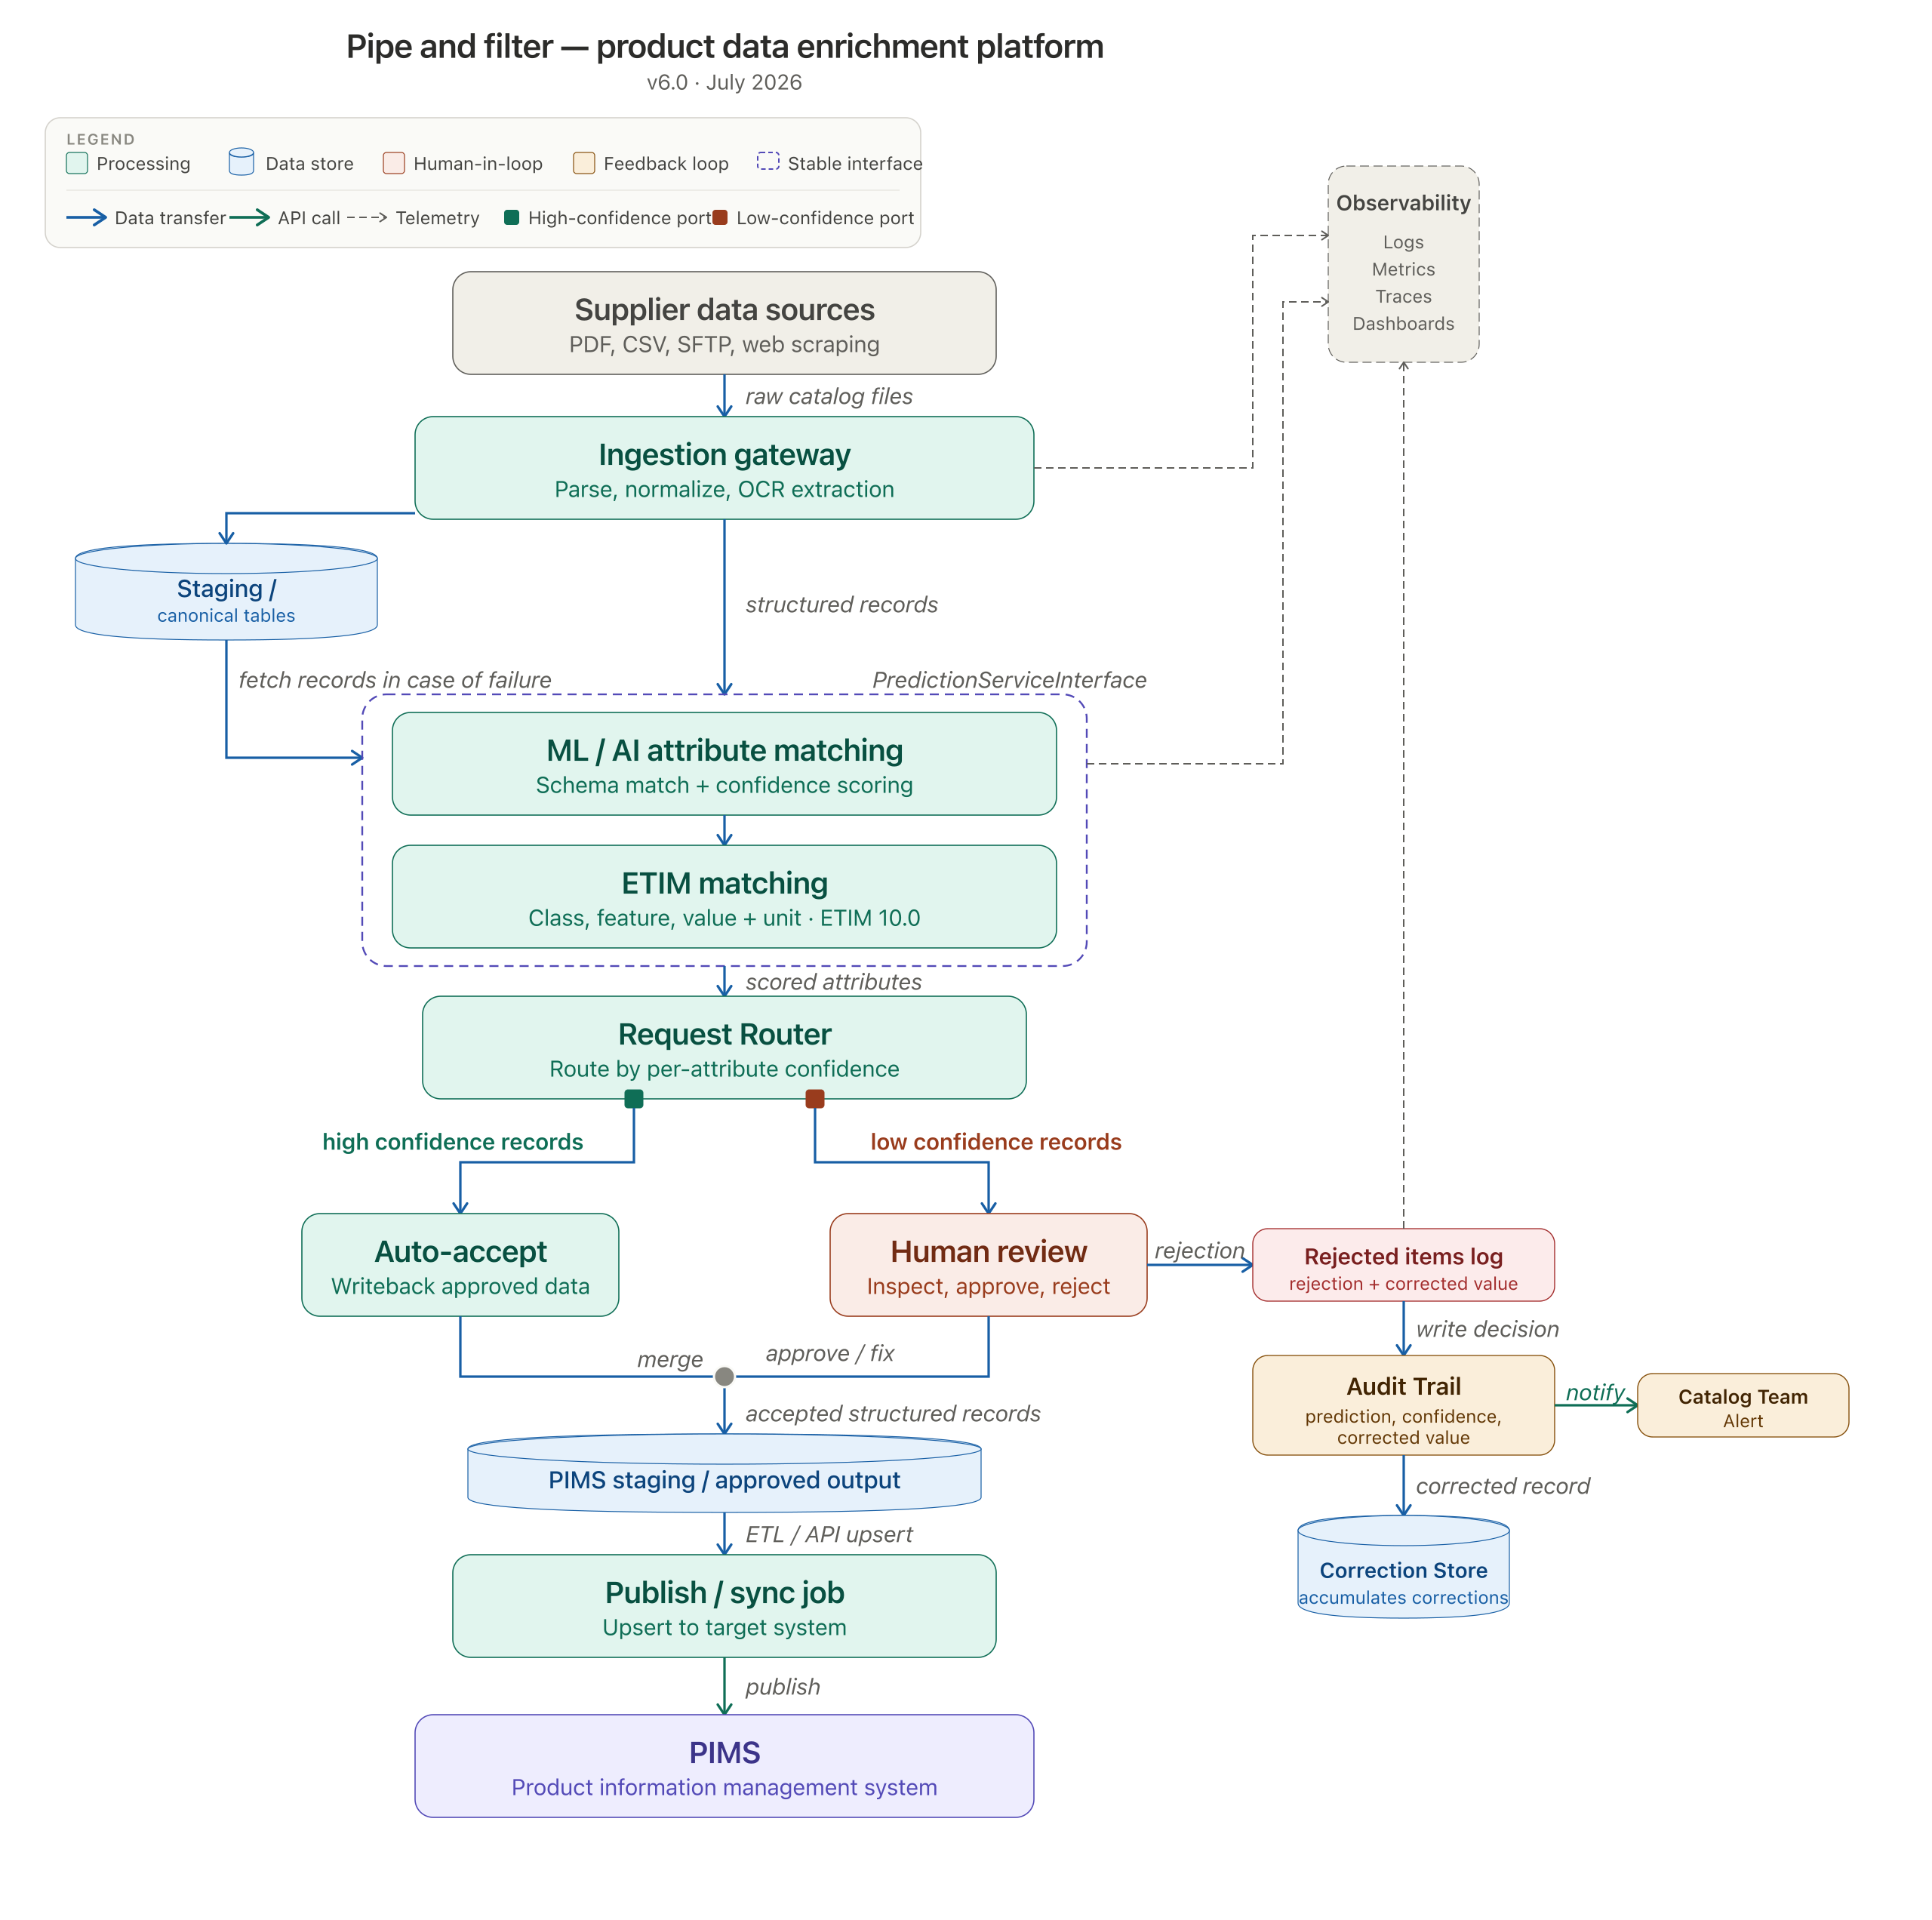
\includegraphics[width=\textwidth]{arch.png}
  \caption{eParts Reference Architecture.}
  \label{fig:architecture}
\end{figure}

\subsection{Component Descriptions}
\begin{itemize}
    \item \textbf{Ingestion Gateway:} Handles "messy" inputs. Identifies submission source, creates ingestion records, and archives raw files to Azure Blob Storage for auditability. Datasheet PDFs are OCR'd via Azure AI Document Intelligence; text-native CSV/PDF are parsed deterministically.
    \item \textbf{Intermediate Structured Layer:} Converts raw inputs into standard, ETIM-keyed canonical tables (class / feature / value), preserving original supplier values as evidence. Supports schema-based transformations.
    \item \textbf{Attribute Prediction Service:} Runs ML models and heuristic rules. Outputs \texttt{{attribute, value, confidence}}.
    \item \textbf{Confidence Routing:} A logic layer that splits traffic. High confidence $\rightarrow$ Auto-Accept. Low confidence $\rightarrow$ Human Review Queue.
    \item \textbf{Engineering Ops / Observability:} Centralized logging (datadog) and metrics to track model drift and ingestion success rates.
\end{itemize}

\newpage
\section{Operational Environment}

\subsection{Cloud Infrastructure}
\begin{itemize}
    \item \textbf{Hosting:} The system shall be hosted on public cloud (Azure) using containerized services (Kubernetes/Docker).
    \item \textbf{Database:} 
    \begin{itemize}
        \item \textbf{Transactional:} PostgreSQL/MSSQL for user accounts, workflow state, and intermediate tables.
        \item \textbf{Data Warehouse:} (Future) for historical model training data.
    \end{itemize}
    \item \textbf{Document Extraction:} Azure AI Document Intelligence (layout OCR) with Azure OpenAI for datasheet attribute extraction.
    \item \textbf{Object Storage:} Azure Blob Storage archives raw supplier files for traceability, accessed through an S3-compatible interface (MinIO in local/dev).
    \item \textbf{Authentication:} Auth0 must be used for all internal user sign-in and role-based access control (RBAC).
\end{itemize}

\subsection{System Constraints}
\begin{tabular}{@{}l >{\raggedright\arraybackslash}p{12cm}@{}}
\toprule
\textbf{ID} & \textbf{Constraint} \\
\midrule
C-1 & \textbf{Cost-Effective Design:} Avoid architectures where cost grows linearly per tenant; prefer shared resources where possible. \\
\addlinespace
C-2 & \textbf{Privacy Compliance:} The system must support data deletion requests (GDPR/CCPA) for specific supplier submissions. \\
\addlinespace
C-3 & \textbf{Breadth-First Delivery:} The initial release must demonstrate a full end-to-end flow for a single supplier type before optimizing model depth. \\
\addlinespace
C-4 & \textbf{ETIM Release Pinned:} The system shall target ETIM release 10.0 (language EI) for the duration of this project. Adopting later ETIM releases, and migrating already-classified products between releases, are out of scope. \\
\bottomrule
\end{tabular}

\newpage
\section{Requirements}

\subsection{High Level Requirements (HLR)}
\begin{tabular}{@{}lp{12cm}@{}}
\toprule
\textbf{ID} & \textbf{High Level Requirement} \\
\midrule
HLR-1 & The system shall ingest product data from diverse supplier sources (SFTP and direct upload today; Email and web sources planned) in CSV and PDF formats. \\
\addlinespace
HLR-2 & The system shall normalize ingested data into a standardized, ETIM-keyed intermediate structure (mechanical cleanup followed by mapping to ETIM classes, features, and values), preserving original supplier values as evidence. \\
\addlinespace
HLR-3 & The system shall predict product attributes and assign confidence scores using Machine Learning. \\
\addlinespace
HLR-4 & The system shall provide a user interface for human review of low-confidence predictions. \\
\addlinespace
HLR-5 & The system shall write approved data back to the PIMS (Product Information Management System). \\
\addlinespace
HLR-6 & The system shall classify products against the ETIM standard and enrich supplier attributes with ETIM identifiers (class, feature, value, unit), keeping the original values as evidence. \\
\bottomrule
\end{tabular}

\subsection{Functional Requirements (FR)}
% UPDATED: Increased width to p{14cm} to better fill page width
\begin{longtable}{@{}l >{\raggedright\arraybackslash}p{14cm}@{}}
\toprule
\textbf{ID} & \textbf{Requirement (EARS Format)} \\
\midrule
\endfirsthead
\toprule
\textbf{ID} & \textbf{Requirement (EARS Format)} \\
\midrule
\endhead
\bottomrule
\endfoot
\bottomrule
\endlastfoot
FR-1 & Upon receipt of a file via SFTP or direct upload (Email and web ingestion are planned), the Ingestion Gateway shall create an ingestion record containing supplier ID, timestamp, and source channel. \\
\addlinespace
FR-2 & The Ingestion Gateway shall validate basic file integrity (type, size, virus scan) before processing; records that fail validation shall be routed to a quarantine store for triage rather than silently dropped. \\
\addlinespace
FR-3 & The Attribute Prediction Service shall generate a confidence score (0.0 to 1.0) for every predicted attribute. \\
\addlinespace
FR-4 & If a prediction's confidence score is below the configured threshold, the system shall route the item to the Human Review Queue. \\
\addlinespace
FR-5 & The Human Review UI shall display the predicted value alongside the original source snippet (text/image) for verification. \\
\addlinespace
FR-6 & The system shall log every human review action (accept/edit/reject) to an immutable audit trail. \\
\addlinespace
FR-7 & The system shall allow authorized Ops Leads to adjust the confidence threshold for auto-acceptance. \\
\addlinespace
FR-8 & Upon final approval (auto or human), the system shall write the attributes to PIMS via API. \\
\addlinespace
FR-9 & The system shall match normalized attributes to ETIM classes, features, and controlled values/units, attaching a confidence score to each ETIM assignment and preserving the original supplier value. \\
\addlinespace
FR-10 & The system shall load and maintain the ETIM reference dictionary (product groups, classes, features, values, units, and class--feature--value mappings) as reference data for the pinned ETIM release identified in C-4. \\
\end{longtable}

\subsection{Derived Requirements (DR)}
\begin{tabular}{@{}l l >{\raggedright\arraybackslash}p{8cm} l@{}}
\toprule
\textbf{ID} & \textbf{Priority} & \textbf{Requirement} & \textbf{Trace} \\
\midrule
DR-1 & Must & The system shall archive the original raw file in Azure Blob Storage as "evidence" for audit purposes even after processing. & HLR-1 \\
\addlinespace
DR-2 & Should & The system shall support manual triggering of model retraining using corrected data from the Review Queue. & HLR-3 \\
\addlinespace
DR-3 & Must & The Writeback service must be idempotent; retrying a write to PIMS must not create duplicate records. & HLR-5 \\
\addlinespace
DR-4 & Must & Approved data written to PIMS shall be keyed by ETIM identifiers (release, class, feature); the writeback idempotency key shall include these identifiers. & HLR-6 \\
\bottomrule
\end{tabular}

\newpage
\section{Quality Attribute Scenarios}

\subsection*{QAS-1: Modifiability (Extensibility)}
\begin{longtable}{@{}lp{12cm}@{}}
\toprule
\textbf{Attribute} & \textbf{Scenario} \\
\midrule
\textbf{ID} & QAS-1 \\
\textbf{Attribute} & Modifiability \\
\textbf{Source} & Developer \\
\textbf{Stimulus} & A new supplier format (e.g., a new JSON schema) needs to be added to the pipeline. \\
\textbf{Response} & The developer adds a new mapping configuration without rewriting the core pipeline code. \\
\textbf{Measure} & A new supplier format can be integrated and deployed within 4 hours of engineering effort. \\
\bottomrule
\end{longtable}

\subsection*{QAS-2: Usability (Ops Efficiency)}
\begin{longtable}{@{}lp{12cm}@{}}
\toprule
\textbf{Attribute} & \textbf{Scenario} \\
\midrule
\textbf{ID} & QAS-2 \\
\textbf{Attribute} & Usability \\
\textbf{Source} & Ops Reviewer \\
\textbf{Stimulus} & The queue contains 100 low-confidence items requiring review. \\
\textbf{Response} & The UI presents items with "diff" views and hotkeys for acceptance. \\
\textbf{Measure} & The reviewer can process simple accept/reject decisions at a rate of 10 items per minute. \\
\bottomrule
\end{longtable}

\newpage
\section{Operational Scenarios}

\subsection*{[SCEN-1] End-to-End Ingestion (Happy Path)}
\begin{itemize}
    \item \textbf{Objective:} A supplier submits a catalog, and it is processed into PIMS without human intervention.
    \item \textbf{Actors:} Supplier, System
\end{itemize}

\begin{longtable}{@{}llp{2cm}p{8cm}@{}}
\toprule
\textbf{Source} & \textbf{Step \#} & \textbf{Req.} & \textbf{Action} \\
\midrule
Supplier & 1 & - & Uploads a CSV catalog to the designated SFTP folder. \\
System & 2 & FR-1 & Detects file, creates ingestion record, and archives raw file. \\
System & 3 & HLR-2 & Cleans and normalizes CSV columns into the ETIM-keyed Canonical Table (maps to ETIM class/features), retaining original values. \\
System & 4 & FR-3 & ML Service predicts attributes. All confidence scores are $>$ 0.90. \\
System & 5 & FR-8 & Auto-Accept logic triggers. Data is written to PIMS. \\
\bottomrule
\end{longtable}

\subsection*{[SCEN-2] Low Confidence \& Review (Human-in-the-Loop)}
\begin{itemize}
    \item \textbf{Objective:} A messy PDF is ingested, low confidence is flagged, and a human corrects it.
    \item \textbf{Actors:} System, Ops Reviewer
\end{itemize}

\begin{longtable}{@{}llp{2cm}p{8cm}@{}}
\toprule
\textbf{Source} & \textbf{Step \#} & \textbf{Req.} & \textbf{Action} \\
\midrule
System & 1 & FR-1 & Ingests a datasheet PDF; routed to Azure AI Document Intelligence (layout OCR) with LLM extraction. Raw OCR output is noisy. \\
System & 2 & FR-3 & ML Service predicts "Voltage: 12V" with confidence 0.45. \\
System & 3 & FR-4 & Confidence $<$ Threshold (0.80). item routed to Review Queue. \\
Ops User & 4 & FR-5 & Opens Review UI. Sees "12V" predicted but PDF says "24V". \\
Ops User & 5 & FR-6 & Corrects value to "24V" and clicks Approve. Action logged. \\
System & 6 & FR-8 & Validated data "24V" is written to PIMS. \\
\bottomrule
\end{longtable}

\newpage
\section{Design Constraints \& Validation}

\subsection{Design Constraints}
% UPDATED: Adjusted column widths to p{10.5cm} and p{3.5cm} to fill page width
\begin{tabular}{@{}l >{\raggedright\arraybackslash}p{10.5cm} >{\raggedright\arraybackslash}p{3.5cm}@{}}
\toprule
\textbf{ID} & \textbf{Constraint} & \textbf{Source} \\
\midrule
DC-1 & \textbf{Tech Stack:} Backend must be Python based (for ML library compatibility). & Team Charter \\
\addlinespace
DC-2 & \textbf{Auth:} Must use Auth0 for identity management. & Client Req \\
\addlinespace
DC-3 & \textbf{Audit:} Raw files must be preserved in Azure Blob Storage for re-processing and traceability. & Regulatory \\
\bottomrule
\end{tabular}

\subsection{Validation Requirements}
\begin{longtable}{@{}p{2cm} >{\raggedright\arraybackslash}p{3.8cm} >{\raggedright\arraybackslash}p{3.8cm} >{\raggedright\arraybackslash}p{3.8cm}@{}}
\toprule
\textbf{Test ID} & \textbf{Description} & \textbf{Steps} & \textbf{Expected Result} \\
\midrule
VAL-1 & \textbf{Ingestion Trigger} & Upload file to SFTP. & Ingestion record appears in DB within 30 seconds. \\
\addlinespace
VAL-2 & \textbf{Routing Logic} & Mock ML response with Conf=0.2. & Item appears in Human Review Queue. \\
\addlinespace
VAL-3 & \textbf{PIMS Integration} & Approve item in UI. & API call to PIMS returns 200 OK. \\
\bottomrule
\end{longtable}

\end{document}